\documentclass[12pt,a4paper]{article}
\usepackage{amsmath}
\usepackage{tikz}
\usepackage[margin=1in]{geometry}
\usetikzlibrary{shapes.geometric, arrows.meta, positioning}
\usepackage{enumitem}
\usepackage{siunitx}

\pagenumbering{gobble}

\begin{document}

\section*{Simplifying Ratios}
\begin{enumerate}
\item \(14:21\)

\textbf{Solution.} Divide both parts by \(7\):
\[
14:21=2:3.
\]

\item \(24:18:42\)

\textbf{Solution.} Divide all three parts by \(6\):
\[
24:18:42=4:3:7.
\]

\item \(1.5:4.5\)

\textbf{Solution.} Multiply both parts by \(2\), then divide by \(3\):
\[
1.5:4.5=3:9=1:3.
\]

\item \(\frac{2}{3}:\frac{4}{5}\)

\textbf{Solution.} Multiply both parts by the LCM of \(3\) and \(5\), which is \(15\):
\[
\frac{2}{3}:\frac{4}{5}
= \left(\frac{2}{3}\times 15\right):\left(\frac{4}{5}\times 15\right)
=10:12=5:6.
\]

\item White : blue : yellow paint \(=600:250:150\).

\textbf{Solution.} Divide all parts by their HCF, \(50\):
\[
600:250:150=12:5:3.
\]
\end{enumerate}

\section*{Sharing into Ratios}
\begin{enumerate}
\item Share 24 sweets in the ratio \(3:1\).

\textbf{Solution.} Total parts \(=3+1=4\). One part \(=24\div4=6\) sweets.
\[
3\times6=18,\qquad 1\times6=6.
\]
So the two children receive \(18\) sweets and \(6\) sweets.

\item Divide \pounds80 in the ratio \(3:2\).

\textbf{Solution.} Total parts \(=3+2=5\). One part \(=80\div5=16\).
\[
3\times16=48,\qquad 2\times16=32.
\]
So the two people receive \pounds48 and \pounds32.

\item Divide 180 students in the ratio \(2:3:4\).

\textbf{Solution.} Total parts \(=2+3+4=9\). One part \(=180\div9=20\).
\[
2\times20=40,\qquad 3\times20=60,\qquad 4\times20=80.
\]
The groups contain \(40\), \(60\), and \(80\) students.

\item A \(2.4\) m piece of wood is cut in the ratio \(1:2:5\).

\textbf{Solution.} Total parts \(=1+2+5=8\). One part \(=2.4\div8=0.3\) m.
\[
1\times0.3=0.3,\quad 2\times0.3=0.6,\quad 5\times0.3=1.5.
\]
The lengths are \(0.3\) m, \(0.6\) m, and \(1.5\) m.

\item Marbles in the ratio red : blue : green \(=2:5:3\), total 150 marbles.

\textbf{Solution.} Total parts \(=2+5+3=10\). One part \(=150\div10=15\).
\[
\text{red}=2\times15=30,\quad
\text{blue}=5\times15=75,\quad
\text{green}=3\times15=45.
\]
There are \(30\) red, \(75\) blue, and \(45\) green marbles.
\end{enumerate}

\section*{Recipe Questions}
\begin{enumerate}
\item Recipe for 4 servings, need 10 servings.

\textbf{Solution.} Scale factor \(=\frac{10}{4}=\frac52\).

\begin{itemize}
\item Minced beef: \(400\times\frac52=1000\) g \(=1\) kg.
\item Onions: \(2\times\frac52=5\) onions, or \(300\times\frac52=750\) g.
\item Chopped tomatoes: \(400\times\frac52=1000\) g \(=1\) kg.
\item Stock: \(150\times\frac52=375\) ml.
\end{itemize}

\item Cookie recipe makes 15 cookies, need 35 cookies.

\textbf{Solution.} Scale factor \(=\frac{35}{15}=\frac73\).

\begin{itemize}
\item Flour: \(225\times\frac73=525\) g.
\item Butter: \(150\times\frac73=350\) g.
\item Sugar: \(100\times\frac73=\frac{700}{3}=233\frac13\) g.
\item Egg: \(50\times\frac73=\frac{350}{3}=116\frac23\) g of beaten egg, i.e. \(2\frac13\) eggs.
\end{itemize}

\item Dressing recipe for 2 portions, need 7 portions.

\textbf{Solution.} Scale factor \(=\frac72\).

\begin{itemize}
\item Olive oil: \(60\times\frac72=210\) ml.
\item Vinegar: \(30\times\frac72=105\) ml.
\item Mustard: \(10\times\frac72=35\) g.
\item Honey: \(5\times\frac72=17.5\) g.
\end{itemize}

\item Lemonade ratio lemon juice : sugar : water \(=2:1:8\), total \(3.3\) litres.

\textbf{Solution.} Total parts \(=2+1+8=11\).
\[
\text{one part}=\frac{3.3}{11}=0.3\text{ litres}.
\]
\[
\text{lemon juice}=2\times0.3=0.6\text{ L},\quad
\text{sugar}=1\times0.3=0.3\text{ L},\quad
\text{water}=8\times0.3=2.4\text{ L}.
\]

\item Curry recipe for 4 people.

\begin{enumerate}[label=(\alph*)]
\item For 11 people, scale factor \(=\frac{11}{4}\).

Chicken: \(400\times\frac{11}{4}=1100\) g \(=1.1\) kg.

Rice: \(200\times\frac{11}{4}=550\) g.

Coconut milk: \(300\times\frac{11}{4}=825\) ml.

Spices: multiply each of the 6 spice quantities by \(\frac{11}{4}\). If counting spice items, this is \(6\times\frac{11}{4}=16.5\) spice-units.

\item With 600 g of chicken:
\[
\frac{600}{400}=1.5
\]
so the recipe can be scaled by \(1.5\). This serves
\[
4\times1.5=6
\]
people.

\item Using the 600 g chicken, scale factor \(=\frac{600}{400}=\frac32\).

Chicken: \(600\) g.

Rice: \(200\times\frac32=300\) g.

Coconut milk: \(300\times\frac32=450\) ml.

Spices: multiply each spice quantity by \(\frac32\); equivalently, \(6\times\frac32=9\) spice-units.
\end{enumerate}
\end{enumerate}

\section*{Direct Proportion}
\begin{enumerate}
\item 4 pencils cost 96p.

\textbf{Solution.} One pencil costs \(96\div4=24\)p.
\[
7\times24=168\text{ p}=\pounds1.68.
\]

\item A car travels 180 km in 3 hours.

\textbf{Solution.} Speed \(=180\div3=60\) km/h.
\[
60\times7=420\text{ km}.
\]

\item 2 litres of paint covers 15 m\(^2\).

\textbf{Solution.}
\[
\frac{90}{15}=6
\]
so 6 times as much paint is needed.
\[
2\times6=12\text{ litres}.
\]

\item A 2.5 m rope costs \pounds1.35.

\textbf{Solution.} Unit price \(=1.35\div2.5=0.54\) pounds per metre.
\[
3.24\div0.54=6\text{ m}.
\]
Bob bought \(6\) metres of rope.

\item A 1.2 m metal bar has mass 4.5 kg.

\textbf{Solution.} \(80\text{ cm}=0.8\text{ m}\).

Unit mass \(=4.5\div1.2=3.75\) kg/m.
\[
3.75\times0.8=3\text{ kg}.
\]
The bar has mass \(3\) kg.
\end{enumerate}

\section*{Best Buys}
\begin{enumerate}
\item 200 g coffee for \pounds5.40 or 350 g for \pounds8.75.

\textbf{Solution.} Use pence per gram.
\[
540\div200=2.7\text{ p/g},\qquad 875\div350=2.5\text{ p/g}.
\]
The \(350\) g pack is cheaper per gram.

\item Pencils: 12 for \pounds4.80 or 30 for \pounds11.00.

\textbf{Solution.}
\[
480\div12=40\text{ p per pencil},\qquad 1100\div30\approx36.7\text{ p per pencil}.
\]
The pack of \(30\) offers better value per pencil.

\item Milk: 2 litres for \pounds2.85 or 5 litres for \pounds6.50.

\textbf{Solution.}
\[
2.85\div2=1.425\text{ pounds per litre},\qquad 6.50\div5=1.30\text{ pounds per litre}.
\]
The \(5\) litre bottle is the better buy.

\item Rice options:
A: 8 kg for \pounds24.80,
B: 15 kg for \pounds44.25,
C: 25 kg for \pounds72.50.

\textbf{Solution.}
\[
A:\ 24.80\div8=3.10\text{ pounds per kg},
\]
\[
B:\ 44.25\div15=2.95\text{ pounds per kg},
\]
\[
C:\ 72.50\div25=2.90\text{ pounds per kg}.
\]
Option C offers the best value per kilogram.

\item Car rental:
X: \pounds45 per day, unlimited mileage.
Y: \pounds35 per day plus \pounds0.15 per mile.
Plan: 250 miles over 3 days.

\textbf{Solution.}
\[
\text{Company X cost}=45\times3=135\text{ pounds}.
\]
\[
\text{Company Y cost}=35\times3+0.15\times250=105+37.5=142.5\text{ pounds}.
\]
Company X is the better deal by \pounds7.50.
\end{enumerate}

\section*{Scaling}
\begin{enumerate}
\item Scale 1:100, wall drawn 3.5 cm.

\textbf{Solution.}
\[
3.5\times100=350\text{ cm}=3.5\text{ m}.
\]

\item Map scale 1:50,000, towns 8.4 cm apart.

\textbf{Solution.}
\[
8.4\times50000=420000\text{ cm}=4.2\text{ km}.
\]

\item Garden drawn to scale 1:20, drawing measures 4 cm by 3 cm.

\textbf{Solution.}
\[
4\times20=80\text{ cm},\qquad 3\times20=60\text{ cm}.
\]
The actual garden is \(80\) cm by \(60\) cm, or \(0.8\) m by \(0.6\) m.

\item Actual car \(4.2\) m, model \(28\) cm.

\textbf{Solution.}
\[
4.2\text{ m}=420\text{ cm}.
\]
\[
28:420=1:15.
\]
The scale is \(1:15\).

\item Map scale: 4 cm represents 5 km.

\begin{enumerate}[label=(\alph*)]
\item Cities \(15.2\) cm apart on the map.
\[
15.2\div4=3.8,\qquad 3.8\times5=19\text{ km}.
\]

\item
\[
4\text{ cm}:5\text{ km}=4:500000=1:125000.
\]

\item The first map has scale \(1:125000\). The other map also has scale \(1:125000\), so neither map shows more detail; they have the same scale.
\end{enumerate}

\item Floor plan \(6\) m by \(4.5\) m, using scale \(1\text{ cm}:1\text{ m}\).

\textbf{Solution.} The drawing should be a rectangle \(6\) cm by \(4.5\) cm.

\begin{center}
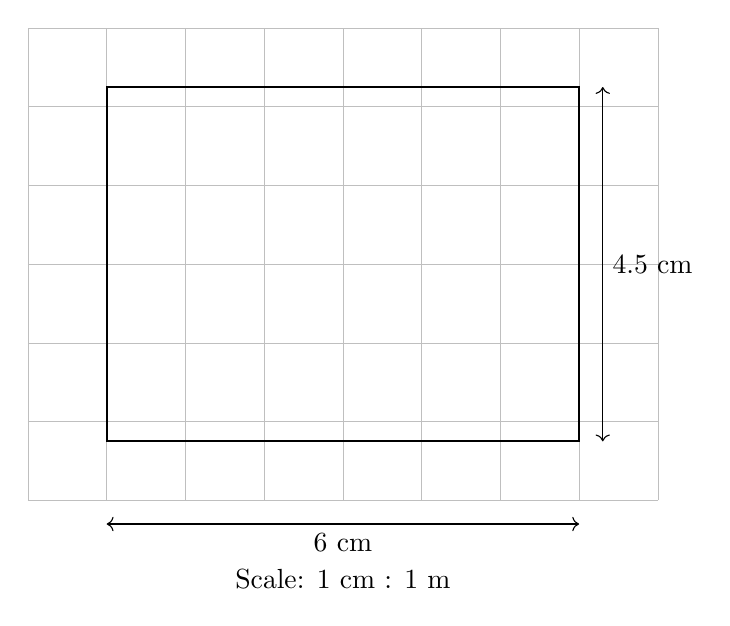
\begin{tikzpicture}
\draw[step=1cm, gray!50, very thin] (0,0) grid (8,6);
\draw[thick] (1,0.75) rectangle (7,5.25);
\draw[<->] (1,-0.3) -- (7,-0.3) node[midway, below] {6 cm};
\draw[<->] (7.3,0.75) -- (7.3,5.25) node[midway, right] {4.5 cm};
\node at (4,-1) {Scale: 1 cm : 1 m};
\end{tikzpicture}
\end{center}
\end{enumerate}

\section*{Rates of Change}
\begin{enumerate}
\item \SI{45}{\kilo\metre} in 1 hour 30 minutes.

\textbf{Solution.} \(1\) h \(30\) min \(=1.5\) h.
\[
45\div1.5=30\text{ km/h}.
\]

\item 12 litres fills in 3 minutes.

\textbf{Solution.} Rate \(=12\div3=4\) L/min.
\[
90\div4=22.5\text{ minutes}=22\text{ minutes }30\text{ seconds}.
\]

\item Train: 320 km, 10:15 to 14:45, with a 10-minute stop.

\textbf{Solution.} Total time from 10:15 to 14:45 is
\[
4\text{ h }30\text{ min}=4.5\text{ h}.
\]
Average speed including the stop:
\[
320\div4.5=71.1\text{ km/h}.
\]
Moving time \(=4.5-\frac{10}{60}=4.5-\frac16=\frac{13}{3}\) hours.
Average speed while moving:
\[
320\div\frac{13}{3}=\frac{960}{13}=73.8\text{ km/h}.
\]

\item Beaker starts with 400 g of chemical A, used at 4 g/min.

\textbf{Solution.} In 4 minutes, used:
\[
4\times4=16\text{ g}.
\]
Remaining:
\[
400-16=384\text{ g}.
\]

\item Sarah drives 30 min at 60 mph, stops 15 min, then drives 45 min at 50 mph.

\begin{enumerate}[label=(\alph*)]
\item First distance:
\[
60\times\frac{30}{60}=30\text{ miles}.
\]
Second distance:
\[
50\times\frac{45}{60}=37.5\text{ miles}.
\]
Total distance:
\[
30+37.5=67.5\text{ miles}.
\]

\item Total time including the stop:
\[
30+15+45=90\text{ min}=1.5\text{ h}.
\]
Average speed:
\[
67.5\div1.5=45\text{ mph}.
\]
\end{enumerate}
\end{enumerate}

\section*{Problem Solving With Ratios}
\begin{enumerate}
\item Red : blue \(=3:5\). After adding 8 red marbles, ratio becomes \(5:7\).

\textbf{Solution.} Let the initial numbers be \(3x\) and \(5x\).
\[
\frac{3x+8}{5x}=\frac{5}{7}
\]
\[
7(3x+8)=25x
\]
\[
21x+56=25x
\]
\[
x=14.
\]
So blue marbles \(=5x=70\).

\item Apples : bananas : oranges \(=2:5:3\). After adding 4 apples and 2 bananas, the ratio becomes \(4:6:3\).

\textbf{Solution.} Let the initial numbers be \(2x,5x,3x\). The number of oranges is unchanged and is still 3 parts in the new ratio, so the new scale is also \(x\).
\[
2x+4=4x \Rightarrow x=2,
\]
and indeed \(5x+2=6x\Rightarrow x=2\). Thus oranges \(=3x=6\).

\item Sugar : flour \(=2:9\), flour : butter \(=3:1\).

\textbf{Solution.} Make the flour part the same.
\[
\text{sugar}:\text{flour}=2:9,
\]
\[
\text{flour}:\text{butter}=3:1=9:3.
\]
Therefore
\[
\text{sugar}:\text{flour}:\text{butter}=2:9:3.
\]

\item Alex : Ben : Chloe \(=3:4:5\). Ben receives \pounds40 more than Alex.

\textbf{Solution.} Let the shares be \(3x,4x,5x\).
\[
4x-3x=x=40.
\]
Total \(=3x+4x+5x=12x=12\times40=480\).
The total sum of money is \pounds480.

\item \(AB:BC=3:2\), \(AB=12\) cm.

\textbf{Solution.} \(AB=3\) parts \(=12\) cm, so one part \(=4\) cm.
\[
BC=2\times4=8\text{ cm}.
\]
\[
AC=AB+BC=12+8=20\text{ cm}.
\]

\item red : yellow \(=3:4\), yellow : blue \(=5:6\).

\textbf{Solution.} Make the yellow part the same.
\[
\text{red}:\text{yellow}=3:4=15:20,
\]
\[
\text{yellow}:\text{blue}=5:6=20:24.
\]
So red : yellow : blue \(=15:20:24\). Total parts \(=15+20+24=59\).
\[
\text{fraction blue}=\frac{24}{59}.
\]

\item Red : blue \(=2:3\). After adding 36 red and 29 blue marbles, the ratio becomes \(4:5\).

\textbf{Solution.} Let initial numbers be \(2x\) and \(3x\).
\[
\frac{2x+36}{3x+29}=\frac45
\]
\[
5(2x+36)=4(3x+29)
\]
\[
10x+180=12x+116
\]
\[
2x=64
\]
\[
x=32.
\]
Initial blue marbles \(=3x=96\).
\end{enumerate}

\end{document}